\addchap{Externes Rahmenprogramm}
Zeitgleich zu unserer KIF ist in Dresden eine Menge los. Dieses Kapitel gibt einen kurzen Abriss der Veranstaltungen, falls ihr uns untreu werden wollt.

\subsection*{Schöne neue Cyberwelt}
Anlässlich der Feierlichkeiten zu 50 Jahre Informatik in Dresden wird eine Ausstellung zum Thema Videospiele im Ratssaal des Fakultätsgebäudes stattfinden.
Die Aufbauten dafür beginnen bereits während der KIF und für KIFfel besteht die Möglichkeit, am Samstag zwischen 10 und 16 Uhr die dort vorbereiteten Exponate zu besichtigen.
Der große Ratssaal befindet sich direkt neben dem Orgabüro im 1. Stock des Andreas-Pfitzmann-Baus.


\subsection*{BRN -- Bunte Republik Neustadt}
Die Bunte Republik Neustadt ist am besten als Stadtteilfest der Neustadt zu beschreiben.
Einwohnern der Neustadt zufolge ist die BRN allerdings gar kein Fest sondern ein Dauerzustand.
Die Feierlichkeiten vom 14. bis 16. Juni sind lediglich eine Jubiläumsveranstaltung.
Für diesen Zeitraum verwandelt sich der Stadtteil in eine große Partyzone.
Überall gibt es Stände mit Essen, Musik und Straßenkünstler sind unterwegs.
Es bot sich an, die Kneipentour parallel zu legen.
Das Programm der BRN findet ihr hier \link{http://brn-programm.de/}.

\subsection*{LNdW -- Lange Nacht der Wissenschaften}
\enquote{Wissenschaft statt Kissenschlacht!}
 Die Lange Nacht der Wissenschaften findet am 14. Juni von 18 bis 1 Uhr statt.
An diesem Abend kann man verschiedene wissenschaftliche Einrichtungen besuchen.
Es gibt diverse Vorträge, Auftritte, offene Labore und es gibt viel auszuprobieren.
Das Programm ist sehr vielfältig und unter \link{http://www.wissenschaftsnacht-dresden.de/programm/} zu finden.

\subsection*{Rammstein}
Am 12. und 13. Juni wird das Rudolf-Harbig-Stadion in Dresden beben.
An diesen beiden Tagen findet dort das Rammsteinkonzert (Europe Stadium Tour 2019) statt.
Wir sind uns sicher, dass es KIFfel gibt, die es geschafft haben, eines der heißbegehrten Tickets zu ergattern, und wünschen viel Spaß.
Der Einlass zur Veranstaltung beginnt dort ab 19 Uhr.

\begin{awesomeblock}[KIFteal]{2pt}{\faQuestion}{KIFteal}
    \textbf{Adresse des Rudolf-Harbig-Stadions:}

    Lennestraße 12

    01069 Dresden
\end{awesomeblock}

\vspace{-10pt}
\begin{center}
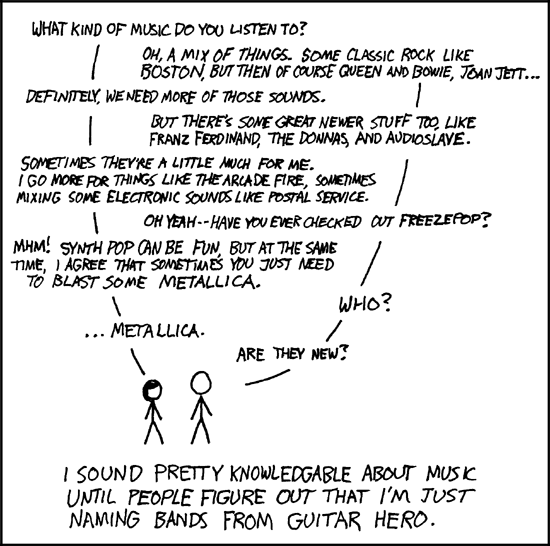
\includegraphics[width=.8\textwidth,keepaspectratio]{img/xkcd/music_knowledge.png}\\
    {\footnotesize \textit{When Guitar Hero 2 comes out I'll have fresh conversational material for MONTHS. (https://xkcd.com/132)}}
\end{center}
